\documentclass[a4paper,10pt,headlines=3.2]{scrartcl}
\usepackage{graphicx}           %Bilder

%\usepackage[T1]{fontenc}        %Umlaute
%\usepackage[latin1]{inputenc}   %Windows
%\usepackage[utf8x]{inputenc}	%Linux
\usepackage{ucs}

\usepackage[ngerman]{babel}     %Deutsche Sprache
\usepackage{amsmath}            %Math. Zeichen
\usepackage{pifont}             %Skalierbare Schriftart
\usepackage{array}
\usepackage{epsfig}             %Erweiterte Grafiken
\usepackage{makeidx}            %Stichwortverzeichnis
\usepackage[pdftex]{color} 

\newcommand{\changefont}[3]{
\fontfamily{#1} \fontseries{#2} \fontshape{#3} \selectfont}

\makeindex

\usepackage[automark]{scrpage2}
\usepackage[nosectionbib]{apacite}               %Zitieren

%\usepackage[colorlinks]{hyperref}%Hyperlinks

\usepackage{lmodern}
\usepackage{scrpage2}           %KOMA-Script
\usepackage{tipa}
\usepackage{qtree}
\usepackage{pgf}


\usepackage{remreset}			%Fussnoten global
\makeatletter
\@removefromreset{footnote}{chapter}
\makeatother 

\setcounter{tocdepth}{3}

%Kopfzeilen
\pagestyle{scrheadings}         %Seitenstil scrheadings verwenden

%\setlength{\textheight}{24cm}
%\setlength{\textwidth}{16cm}
%\setlength{\topmargin}{-2cm}
%\setlength{\oddsidemargin}{0cm}

% Groesse des Textbereiches in der Seite
\setlength{\textwidth}{16cm}
\setlength{\textheight}{22cm}
% Kopf- und Fusszeile, Hoehe und Abstand vom Text
\setlength{\headheight}{15pt}
\setlength{\headsep}{0.8cm}
% Linker Seiteneinzug
\setlength{\oddsidemargin}{2.5cm} \addtolength{\oddsidemargin}{-1in}
\setlength{\evensidemargin}{2.5cm} \addtolength{\evensidemargin}{-1in}
% Andere Groessen ausrechnen (vertikal zentrieren)
\setlength{\footskip}{\headsep}
\addtolength{\footskip}{\headheight}
\setlength{\topmargin}{\paperheight}
\addtolength{\topmargin}{-\textheight}
\addtolength{\topmargin}{-\headheight}
\addtolength{\topmargin}{-\headsep}
\addtolength{\topmargin}{-\footskip}
\addtolength{\topmargin}{-2in}
\addtolength{\topmargin}{-0.5\topmargin}

%Schriftart
\changefont{cmss}{m}{n}

%Abstand zur�cksetzen
\setlength{\headheight}{20pt}

\usepackage{listings} 
\lstset{numbers=left, numberstyle=\tiny, numbersep=5pt} \lstset{language=Java} 

\clearscrheadfoot
%\renewcommand{\headheight}{40pt} 
\ihead[]{Datenstrukturen und Algorithmen \\Fr�hlingssemester 2011 \\Institut f�r angewandte Mathematik} % - links
\ohead[asdasd]{�bung 7 \\Abgabetermin 14. April 2011 \\Adrianus Kleemans [07-111-693]} % - linke Kopfzeile 
\setheadsepline{.4pt} %Separate Linie im Kopf
\cfoot[\pagemark]{\pagemark} %- mittlere Fusszeile 

\begin{document}
\section*{Theoretische Aufgaben: Bin�re Suchb�ume}
\subsection*{Aufgabe 1}
\begin{figure}[ht]
\centering
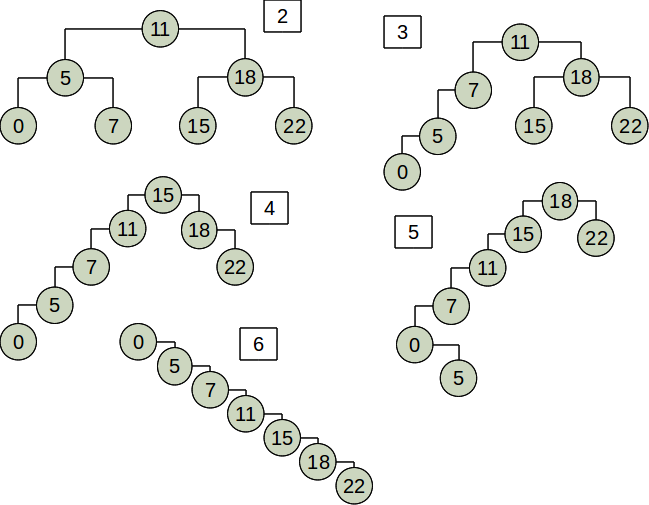
\includegraphics[height=10cm]{aufg1}
\end{figure}
\subsection*{Aufgabe 2}
Min-Heap-Bedingung: Die Schl�ssel der Kinder eines Knotens sind stets gr�sser als der Schl�ssel ihres Vaters.\\
Beim Bin�rbaum sind im Unterschied dazu die Kinder links immer kleiner oder gleich, rechts immer gr�sser oder gleich.\\
Zur sortierten Ausgabe mit Min-Heap: Diese ist nicht m�glich, da zu einem bestimmten Knoten nichts �ber die beiden Teilb�ume ausgesagt werden kann (im Gegenteil zum bin�ren Suchbaum).

\subsection*{Aufgabe 3}

\begin{figure}[ht]
\begin{minipage}[t]{.35\linewidth}
\vspace{0pt}
\centering
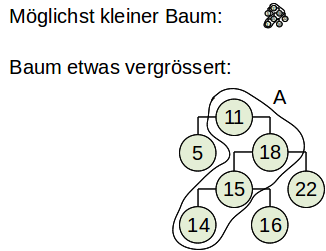
\includegraphics[height=4cm]{aufg3}
\label{fig:Bild1}
\end{minipage}
\hfill
\begin{minipage}[t]{.6\linewidth}
\vspace{0pt}
Im Beispiel sollte das Element mit Schl�ssel 16 laut Behauptung gr�sser sein als z.B. Element mit Schl�ssel 18 auf dem gegangenen Pfad. Dies ist aber nicht der Fall, deshalb kann die Behauptung nicht stimmen.
\end{minipage}
\end{figure}

\subsection*{Aufgabe 4}
Definition des Nachfolgers: Das im Sortierkriterium n�chstfolgende Element. Definition von linkem Teilbaum: Element muss kleiner gleich dem Vater sein. Schluss: Der Nachfolger von $x$ kann kein linkes Element haben, da dies zwischen den Elementen w�ren. Dies zerst�rte die Reihenfolge, der fr�here Nachfolger von $x$ w�re nicht mehr der Nachfolger.\\
Nimmt man an, es g�be ein linkes Kind vom Nachfolger von $x$. dieses m�sst in der Reihenfolge der Sortierung vor dem Nachfolger von $x$ liegen. Da dies nicht $x$ ist, und $x$ schon als Vorg�nger definiert ist, ergibt sich ein unl�sbarer Widerspruch; Es kann kein linkes Kind geben. Analog gilt dies auch f�r den Vorg�nger von $x$, der kein rechtes Kind haben kann.

\subsection*{Aufgabe 5}
\lstset{frame=single}
\begin{lstlisting}[caption=Aufgabe 5]{Name}
treesort (array numbers)

for i = 0 to numbers.size()
  tree-insert(numbers[i])

traverse(numbers)
\end{lstlisting}

Laufzeiten
\begin{itemize}
 \item Best Case: H�he des Baumes: $\Theta(lg\, n)$, ausgeben $\Theta(n)$ $\Rightarrow \Theta(n \cdot lg\, n)$
 \item Worst Case: H�he des Baumes: $\Theta(n)$, ausgeben: $\Theta(n)$ $\Rightarrow \Theta(n^2)$
\end{itemize}


\section*{Theoretische Aufgaben: Repetition}
\subsection*{Aufgabe 1}
\begin{lstlisting}[caption=Aufgabe 1]{Name}
concatenate (nil[a], nil[b])

//temporary variables
t1 = next[nil[b]]
t2 = last[nil[b]]

//if nil[b] doesn't point to itself,
//readress pointers
if t1 != nil[b]
  next[last[nil[a]]] = t1 //point to beginning of b
  last[t1] = last[nil[a]] //link to last element of a
  next[t2] = nil[a]       //close circle
  last[nil[a]] = t2       
\end{lstlisting}

\subsection*{Aufgabe 2}
(a) $\Theta(2^n)$, (b) $\Theta(n^5)$, (c) $\Theta(n)$, (d) $\Theta(n)$, (e) $\Theta(n)$, (f) $\Theta(n^4)$, (g) $\Theta(n\cdot log\, n)$, (h)$\Theta(n\cdot log\, n)$, (i) $\Theta(1)$\\\\
Reihenfolge: $\{i, e, c, d, g, h, f, b, a\}$

\subsection*{Aufgabe 3}
Der Algorithmus hat eine Laufzeit von $\Theta(n)$. Bis auf den ersten Durchlauf wird in jedem folgenden Durchlauf zuerst die Variable $j$ erh�ht, die innere Schleife bricht ab, $i$ wird erh�ht, und die �ussere Schleife beginnt von vorne.
\begin{lstlisting}[caption=Aufgabe 3]{Name}
i,j = 1
while i <= n
  while j <= i + 5
    j=j+1
  i=i+1
\end{lstlisting}

\subsection*{Aufgabe 4}
-

\subsection*{Aufgabe 5}
\begin{lstlisting}[caption=Aufgabe 5]{Name}
minPrice(i, length, min)

if length < 0 return 0 //keine Kombination
if length > n return 0 //alle Platten durchsucht
if l = 0 return min    //L�sung gefunden

//Keine der bisherigen F�lle, schaue weiter
min1 = minPrice(i+1, length-length(i), min+price(i))
min2 = minPrice(i+1, length, min)

if min1 < min2 return min1
else return min2
\end{lstlisting}

\end{document}